%Erstemal, dass ich mit Latex arbeite, daher bitte nicht schlagen :D
\documentclass[a4paper, 11pt]{report}

\usepackage[ngerman]{babel}
\usepackage[latin1]{inputenc}
\usepackage{graphicx}
\usepackage{amsmath}
\usepackage{txfonts}
\usepackage{pstricks}

\newcommand{\N}{\varmathbb{N}}
\newcommand{\Z}{\varmathbb{Z}}
\newcommand{\Q}{\varmathbb{Q}}
\newcommand{\R}{\varmathbb{R}}
\newcommand{\C}{\varmathbb{C}}
\begin{document}

\tableofcontents

\newpage
\chapter{Einf�hrung}
\section{Inhalt}
�bertragung (Speicherung) von Daten:\\
Schutz vor:
\begin{itemize}
	\item[-] zuf�lligen oder systematischen (physikalischen bedingten) St�rungen
	\item[-] Abh�ren, absichtliche Ver�nderung von Dritten (Kryptologie / Verschl�sselung)
\end{itemize}
\underline{Kryptologie:}
\begin{itemize}
	\item[-] symmetrische Verfahren
	\item[-] asymmetrische Verfahren (Public-Key Verfahren)
	\item[-] Authentifizierung
	\item[-] Signaturen
\end{itemize}
\underline{Codierungstheorie}
\begin{itemize}
	\item[-] Fehlererkennung und Fehlerkorrektur
	\item[-] lineare Blockcodes
	\item[-] Decodierverfahren
\end{itemize}	%Einf�hrung
\chapter{Kryptologie}

\section{Grundbegriffe und einfache Verfahren}
\begin{figure}[h]
	\centering
	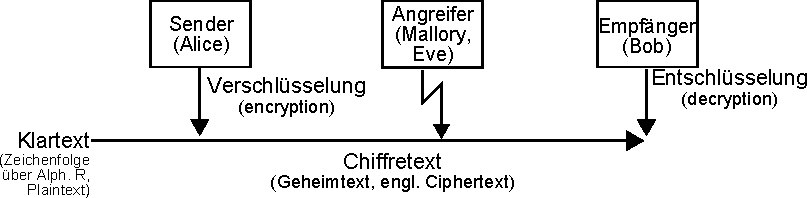
\includegraphics{./img/krypto_schaubild.pdf}
	\caption{Schaubild der Kryptologie}
	\label{img:Schaubild}
\end{figure}

\subsection{Verschl�sselung erfordert}

\begin{itemize}
	\item[-] Verschl�sselungsverfahren, Algorithmus (Funktion)
	\item[-] Schl�ssel $k_{e}$ (encryption key)
\end{itemize}

\[
	E(m,k_e)=c
\]	
$E$=Verschl�sselungs Funktion, $m$=Klartext, $c$=Chiffretext
\[
	E(m_1,k_e) \neq E(m,k_e)\ fuer \ m_1 \neq m_2
\]
\[
	D(c,k_d)=m
\]	
($k_d$ zu $k_e$ geh�riger Dechiffrierschl�ssel!)\\
$k_d=k_e$ (oder $k_d$ leicht aus $k_e$ zu berechnen):\\
\textbf{symmetrisches Verschl.verf.}, ansonsten \textbf{asymm. Verschl.verf.}. Ist $k_d$ nur sehr schwer (oder garnicht) zu $k_e$ berechenbar, so kann $k_e$ ver�ffentl. werden:\\
\textbf{Public-Key-Verfahren}.

\subsection{Beispiel f�r (nicht sicheres) symm. Verfahren}

\begin{itemize}
	\item[a)] $R=S=\left\{0,1,\ldots,25\right\}$\\
	Verfahren: Verschiebechiffre\\
	Schl�ssel: $i \in \left\{0,1,\ldots,25\right\}$\\
	Verfahren $ x \in \R \longrightarrow x+i\, mod\, 26=y$\\
	$y\longmapsto y-i\, mod\, 26 = y$\\
	$m=x_1 ... x_2 \longrightarrow  c = (x_1 + i\, mod\, 26) \textbf{}\ldots (x_n +i\, mod\, 26)$, $E(m,i)$\\
	Unsicher, weil Schl�sselmenge klein ist (Brute Force Angriff).
	\item[b)] R,S, Schl�sselmenge=Menge aller Permutationen von $\left\{1,\ldots,25\right\}=S_{26}$\\
	Verschl.: W�hle Permuation $\pi$\\
	$x \in \R \longrightarrow \pi (x)=y$\\
	Entschl.: $y \longrightarrow \pi^{-1}(y)=x$\\
	$m=x_1 \ldots x_r \rightarrow c=\pi(x_1)\ldots\pi(x_r)$\\
	$\begin{pmatrix}
  0 & 1 & 2 & \ldots & 25 \\
  3 & 17 & 4 & \ldots & 13
	\end{pmatrix}
	\longrightarrow \pi(0)=3$, u.s.w.\\
	Anzahl der Permutationen: $\left|{S_{26}}\right|=26!\approx4\cdot10^{26} \longrightarrow$ Brute-Force Angriff nicht mehr m�glich! \\
	Warum? Man muss im Schnitt 50\% der Permutationen testen. Angenommen man k�nnte $10^12$ Perm. pro Sekunde testen.\\
	Aufwand: $2\cdot10^{14}$ Sekunden $\approx 6.000.000$ Jahre\\
	Trotzdem unsicher!\\
	Grund: Charakteristiches H�ufigkeitsverteilung von Buchstaben in nat�rlichspr. Texten.
\end{itemize}
Verfahren beinhalten viele Verschl�sselungsm�glichkeiten, abh�ngig von der Auswahl des Schl�ssels.\\
Verfahren bekannt, aber Schl�ssel $k_d$ geheim!\\
\subsection{Prinzip von Kerkhoffs (1835-1903)}
Sicherheit eines Verschl�sselungsverfahren darf nicht von der Geheimhaltung des Verfahrens, sondern nur von der Geheimhaltung des verwendeten Schl�ssels abh�ngen!
%
%	Ende Stunde vom 29.10.2009
%
\\\\
Kryptologie besteht aus Kryptographie (Entwurf) und der Kryptoanalyse (Angriff).
Angriffserfolge:
\begin{itemize}
	\item[-] Schl�ssel $k_d$ wird gefunden
	\item[-] Eine zu der Dechiffrierfunktion $D(\cdot,k_d)$ �quivalente Funktion finden ohne Kenntnis von $k_d$
	\item[-] gewisste Chiffretexte werden entschl�sselt
\end{itemize}
\subsection{Arten von Angriffen}
\begin{itemize}
	\item[-] Ciphertext-Only Angriff
	\item[-] Known-Plaintext Angriff
	\item[-] Chosen-Plaintext Angriff
	\item[-] Chosen-Ciphertext Angriff
\end{itemize} %Kryptologie
\chapter{One-Time-Pad und perfekte Sicherheit}

Lauftextverschl�sselung
\\
Alphabet $\Z_k=\{0,1,\ldots,k-1\}$\\
In $\Z_k$ kann man addieren und multiplizieren mit $mod\,k$.\\
Klartext $x_1,x_2,\ldots,x_n$\\
Schl�sselwort $k_1,k_2,\ldots,k_n$\\
$x_1 + k_1\, mod\, k$, $x_n + k_n\, mod\, k \leftarrow$ Chiffretext\\
Mit nat�rlichsprachlichen Texten ist das Verfahren unsicher.\\
$\Z_2=\{0,1\}$, $1 \oplus 1 = 0 = 0 \oplus 0$, $0 \oplus 1 = 1 = 1 \oplus 0 \Rightarrow XOR$\\
Klartext in $\Z_2^n=\{(x_1,\ldots,x_n):x_i \in \Z_2\}$
Schl�ssel: Zufallsfolge �ber $\Z_2$ der L�nge $n$. $m$ Klartext, $k$ Zufallsfolge (beide L�nge $n$)\\
$c=m\oplus k$, $(x_1,\ldots,x_n)\oplus(k_1,\ldots,k_n):=(x_1\oplus k_1,\ldots,x_n\oplus k_n)$\\
\section{One-Time-Pad}
Schl�ssel $k$ darf nur einmal verwendet werden!\\
\[
	m_1\oplus k=c_1, m_2 \oplus k=c_2,c_1\oplus c_2=m_1\oplus k \oplus m_2\oplus k=m_1\oplus m_2
\]
Wieder nur Lauftext $\rightarrow$ unsicher!\\
$m_1$ und $m_2$ l�sst sich ermitteln.\\
Zufallsfolge der L�nge $n$: eigentlich unsinniger Begriff. Da jedes Bit unabh�ngig von anderen mit Wahrscheinlichkeit $\frac{1}{2}$ erzeugt wird (Output einer bin�r symmetrischen Quelle)\\
Jede Folge der L�nge $n$ ist gleich wahrscheinlich (Wahrscheinlichkeit $\frac{1}{2} n$\\
One-Time-Pad ist perfekt sicher.
\section{Perfekte Sicherheit}
Ein Verschl�sselungsverfahren ist perfekt sicher, falls gilt: F�r jeden Klartext $m$ und jedem Chiffretext $c$ (der festen L�nge $n$)\\
$pr(m|c)=pr(m)$\\
$pr(m|c)\rightarrow$ A-posteriori-Wahrscheinlichkeit (Wahrscheinlichkeit, dass $m$ Klartext, wenn $c$ empfangen wurde)\\
$pr(m)\rightarrow$ A-priori-Wahrscheinlichkeit\\
\textbf{Beispiel:} Substitutionschiffre aus Kapitel 2.\\
$n=5, m=HALLO, pr(m)>0$\\
Ang:$c=QITUA$ wird empfangen, $LL\neq TU \rightarrow pr(m|c)=0$\\
nicht perfekt sicher.\\
One-Time-Pad ist perfekt sicher. \\
(Bayes'sche Formel) $m\oplus k$\\
Jede Folge $c$ l�sst sich mit geeignetem $k$ in der Form $c=m\oplus k$ erhalten.\\
W�hle $k=m\oplus c$, $m\oplus k=m\oplus m \oplus c=c$\\
Bei gegebenem $m$ und zuf�llige gew�hlten Schl�ssel $k$ ist jeder Chiffretext gleichwertig. %One-TimePad und perfekte Sicherheit
\chapter{Symmetrische Blockchiffre}
\section{Blockchiffre}
Zerlege Klartext in Bl�cke (Strings) der L�nge $n$.  Jeder Block wird einzeln verschl�sselt (in der Regel wieder in einem Block der L�nge $n$). Gleiche Bl�cke werden gleich verschl�sselt.\\
Wieviele Blockchiffren der L�nge $n$ gibt es?\\
Alphabet $\Z_2=\{0,1\}$\\
$|\{\underbrace{(0,\ldots,0)}_{Block},(0,\ldots,1),\ldots,(1,\ldots,1)\}| = 2^n$\\
Blockchiffre = Permuation der $2^n$ Bl�cke.\\
$(2^n)!$ Blockchiffre\\
Wenn alle verwendet werden:\\
Schl�ssel = Permuation der $2^n$ Bl�cke\\
$(x_{1,1},\ldots,x_{1,n},x_{2,1},\ldots,x_{2,n},\ldots)$ \ \ \fbox{$n\cdot 2^n$ Bit}\\
Zur Speicherung eines Schl�ssels werden $n \cdot 2^n$ Bit ben�tigt.\\
Zum Beispiel:\\
$n=64, \ 64 \cdot 2^{64}=2^{70}\approx$ 1 ZetaByte $\approx$ 1 Milliarde Festplatten � 1 TB\\
\textbf{Illusional!}\\
Konsequenz:\ Verwende Verfahren, wo nur ein kleiner Teil der Permutation als Schl�ssel verwendet wird und so sich die Schl�ssel dann in k�rzerer Fom darstellt.
%
% Ende zweiter Vorlesung
% %Symmetrische Blockchiffre
\chapter{Affin-lineare Chiffre}

\section{Vorbemerkung}

\subsection{$n\times m$-Matrix}

\[
\begin{pmatrix}
	a_{11} & \ldots & a_{1m} \\
	\vdots &  & \vdots \\
	a_{n1} & \ldots & a_{nm}
\end{pmatrix}
\]

$1 \times n$ = Zeilenvektor = $(a_1,\ldots,a_m)$

$n \times 1$ = Spaltenvektor = $\begin{pmatrix} b_1 \\ \vdots \\ b_n \end{pmatrix}$

z.B. $a_{ij} \in \R,\ a_{ij} \in \Z$ oder $a_{ij} \in R,\ R$ Ring

$n \times m$-Matrix A,B
\[
\begin{pmatrix}
	a_{11} & \ldots & a_{1m} \\
	\vdots &  & \vdots \\
	a_{n1} & \ldots & a_{nm}
\end{pmatrix}
+
\begin{pmatrix}
	b_{11} & \ldots & b_{1m} \\
	\vdots &  & \vdots \\
	b_{n1} & \ldots & b_{nm}
\end{pmatrix}
:=
\begin{pmatrix}
	a_{11}+b_{11} & \ldots & a_{1m}+b_{1m} \\
	\vdots &  & \vdots \\
	a_{n1}+b_{n1} & \ldots & a_{nm}+b_{nm}
\end{pmatrix}
\]
\[
A=n\times m,\ B = m \times k,
\]
\[
A \cdot B
\begin{pmatrix}
	c_{1l} & \ldots & c_{1k} \\
	\vdots &  & \vdots \\
	c_{m1} & \ldots & c_{mk}
\end{pmatrix}
=
n\times k
\]
\[
c_{1l}=(a_{i1} \cdot b_{ij})+(a_{i2} \cdot b_{2j}) + \ldots + (a_{im} \cdot b_{mj})
\]
\[
(A+B)\cdot C = A\cdot B + B\cot C
\]

Im Allgemeinem: $A\cdot B \neq B\cdot A$\\

\subsection{Quadritsche Matrix ($n\times n$)}

\[
E_n=\begin{pmatrix}
	1 & \ldots & 0 \\
	\vdots & \ddots & \vdots \\
	0 & \ldots & 1
\end{pmatrix}
\]
\[
A=n\times n,\ A \cdot E_n=E_n \cdot A = A
\]
$A\ n\times n$-Matrix �ber kommutativen Ring R mit Eins.\\
Wann existiert Matrix $A^{-1}$(Inverse Matrix) mit $A^{-1} \cdot A = A \cdot A^{-1} = E_n$?\\
$det(A) \in R$\ Determinante von A\\
\\
$2\times 2$-Matrix: $det\begin{pmatrix}
	a_{11} & a_{12} \\ a_{21} & a_{21}
\end{pmatrix}
= a_{11} \cdot a_{22} - a_{12} \cdot a_{21}$\\
\\
\\
A besitzt inverse Matrix $\Leftrightarrow det(A)$ in R ein inverses besitzt\\
(z.B. R K�rper, $\Z ,\Q ,\Z_p,\ det(A)\neq 0$\\
\[
A^{-1}=
\begin{pmatrix}
	\frac{1}{det(A)}\cdot b_{11} & \ldots & \frac{1}{det(A)}\cdot b_{1m} \\
	\vdots & & \vdots \\
	\frac{1}{det(A)}\cdot b_{n1} & \ldots & \frac{1}{det(A)}\cdot b_{nm}
\end{pmatrix}
\]
$b_{ij}=(-1)^{i+j}$\ $det(A_{ji})$\\
\\
$A_{ji}=(n-1)\times (n-1)$-Matrix, die aus $A$ durchstreichen der $j$-ten Zeile und $i$-ten Spalte entsteht.
\[
A=
\begin{pmatrix}
	a_{11} & a_{12} \\ a_{21} & a_{22}
\end{pmatrix}\ \
A^{-1}=
\begin{pmatrix}
	a_{22} & -a_{12} \\ -a_{21} & a_{11}
\end{pmatrix}
\]
$R=\Z_k \ \{0,1,\ldots,k\}$\\
Addition und Multiplikation in $\Z_k (\oplus,\odot)$\\
normale Add. und Mult. mit $mod\, k$\\

\section{Affin-lineare Chiffren}
Klartextalphabet = Chiffretextalphabet = $\Z_k$ ($k=2,\ k=26$)\\
W�hle $n \times n$-Matrix $A$ �ber $\Z_k$ und Zeilenvektor $b$ der L�nge $n$ �ber $\Z_k$. Dies wird der Schl�ssel sein f�r die Chiffrierung.\\
Blockchiffre der L�nge $n$. Block = Zeilenvektor der L�nge $n$ �ber $\Z_k$.
Klartextblock $v$\\
Chiffretextblock $v \cdot A + b =: w$\\
$v \rightarrow v \cdot A +b =:w$
$w-b=v \cdot A$
ben�tigen: $A^{-1}$ existiert (d.h. $ggT(det(A),k)=1$)\\
Dechiffrierung: $(w-b)\cdot A^{-1} = v \cdot A \cdot A^{-1} = v \cdot E_n = v$\\
(wenn immer b=0 gew�hlt wird, dann lineare Chiffren, Hill-Chiffren)\\
Beispiel:\\
\[
A=
\begin{pmatrix}
	1 & 3 \\ 3 & 2
\end{pmatrix}
\ \Z_6
\]
Blockchiffre der L�nge $n$
$det(A)=1 \cdot 2 - 3 \cdot 3 = -7 = 5$ inverse in $\Z_6$
\[
\frac{1}{det(A)}=det(A)^{-1}=5
\]
\[
A^{-1}=5\cdot
\begin{pmatrix}
	2&-3\\-3&1
\end{pmatrix}
=
\begin{pmatrix}
	10&-15\\-15&5
\end{pmatrix}
=
\begin{pmatrix}
	4&3\\3&5
\end{pmatrix}
\]
Test: 
\[
A \cdot A^{-1} = 
\begin{pmatrix}
	1 & 3 \\ 3 & 2
\end{pmatrix}
\cdot
\begin{pmatrix}
	4&3\\3&5
\end{pmatrix}
=
\begin{pmatrix}
	4+9&3+15\\12+6&9+10
\end{pmatrix}
=
\begin{pmatrix}
	1&0\\0&1
\end{pmatrix}
\]
Verschl�sselung:

Schl�ssel:
$A = 
\begin{pmatrix}
	1 & 3 \\ 3 & 2
\end{pmatrix}
$ $b=(3,5)$

Klartextblock: $(1,2)$

Chiffretextblock: 
\[w=(1,2) \cdot 
\begin{pmatrix}
	1 & 3 \\ 3 & 2
\end{pmatrix}
+
(3,5)= (1,1)+(3,5) = (4,0)\]

Entschl�sselung:
\[ (w-b) \cdot A^{-1} = (1,1) \cdot 
\begin{pmatrix}
	4 & 3 \\ 3 & 5
\end{pmatrix}
=(1,2)
\]

$\Z_2 : n^2 + n$ Bit zur Speicherung eines Schl�ssels.

Wieviele inverse Matrizen �ber $\Z_2$ mit $n=64$?

$(2^{64}-1) \cdot (2^{64}-2) \cdot \ldots \cdot (2^{64}-2^{63}) \approx 0.29 \cdot 2^{4096}$

Verfahren ist unsicher gegen�ber Known-Plaintext-Angriffe.

$(A,b)$ Schl�ssel, A inverse $n \times n$-Matrix �ber $\Z_k ,b \ \in \Z_k^n$

Angenommen Angreifer kennt $n+1$ Klartext/Chiffretextpaare verschl�sselt mit $(A,b),\ v_0, v_1,\ldots,v_n \ w_0,\ldots,w_n$

Dann kann er haufig $(A,b)$ bestimmen.

$V=
\begin{pmatrix}
	v_1-v_0\\v_2-v_0\\\vdots\\v_n-v_0
\end{pmatrix}
\ n \times n$-Matrix

Angenommen: V ist invertierbar. Setze $W=
\begin{pmatrix}
	w_1-w_0\\\vdots\\w_n-w_0
\end{pmatrix}$
\[
V \cdot A =
\begin{pmatrix}
	(v_1-v_0) \cdot A \\ \vdots \\(v_n-v_0) \cdot A
\end{pmatrix}
=
\begin{pmatrix}
	v_1 \cdot A + b - v_0 \cdot A +b \\ \vdots \\
	v_n \cdot A + b - v_0 \cdot A + b
\end{pmatrix}
=
\begin{pmatrix}
	w_1-w_0\\ \vdots\\w_n-w_0
\end{pmatrix}
=W
\]

$V \cdot A$ bekannt, also auch $V^{-1}$:

$A=V^{-1} \cdot w$

$b=w_0 - v_0 \cdot A$

Beispiel: $n=2,\ k=25 \ \ \{A,\ldots, Z\}=\{0,\ldots,25\}$

\begin{center}
\texttt{HERBST} $\longrightarrow$ \texttt{NEBLIG}

\begin{tabular}{l|l|l}
H & 7 & \multirow{2}{*}{$v_0$} \\
E & 4 & \\
\hline
R & 17 & \multirow{2}{*}{$v_1$} \\
B & 1 & \\
\hline
S & 18 & \multirow{2}{*}{$v_2$} \\
T & 19 &
\end{tabular}
$\longrightarrow$
\begin{tabular}{l|l|l}
N & 13 & \multirow{2}{*}{$w_0$} \\
E & 4 & \\
\hline
B & 1 & \multirow{2}{*}{$w_1$} \\
L & 11 & \\
\hline
I & 8 & \multirow{2}{*}{$w_2$} \\
G & 6 &
\end{tabular}
\end{center}
\[
V=
\begin{pmatrix}
	10 & -3 \\
	11 & 15
\end{pmatrix}
=
\begin{pmatrix}
	10 & 23\\
	11 & 15
\end{pmatrix}, \
W=
\begin{pmatrix}
	14 & 7 \\
	21 & 2
\end{pmatrix}
\]
\[
det(V) = 10 \cdot 15  + 33 = 183 \equiv 1 (mod\ 26)
\]
\[
V^{-1}=
\begin{pmatrix}
	15 & 3 \\
	-11 & 10 	
\end{pmatrix}
=
\begin{pmatrix}
	15 & 3 \\
	15 & 10 	
\end{pmatrix}
\]
\[
A=V^{-1} \cdot W =
\begin{pmatrix}
	15 & 3 \\
	15 & 10 	
\end{pmatrix}
\cdot
\begin{pmatrix}
	14 & 7 \\
	21 & 2
\end{pmatrix}
=
\begin{pmatrix}
	210+63 & 105+6 \\
	210+210 & 105+20
\end{pmatrix}
=
\begin{pmatrix}
	13 & 7\\
	4 & 21
\end{pmatrix}
\]
\[
b=w_0-v_0 \cdot A = (13,4) - (7,4) \cdot 
\begin{pmatrix}
	13 & 7\\
	4 & 21
\end{pmatrix}
=
(10,1)
\]

Test:
\[
v_1 \cdot A + b= w_1, v_2 \cdot A + b= w_2
\]
 %Affin-Lineare Chiffre


\chapter{Secret Sharing}
Geheimnis wird auf mehrere Teilnehmer verteilt (Teilgeheimnisse), so dass gewisse Teilmengen der Teilnehmer das Geheimnis mit ihren Teilgeheimnissen rekonstruieren k�nnen, die anderen nicht. \\ \\
$T$ = \{ $t_1, \ldots , t_n$\}, $k < n$ \ \ (T Menge der Teilnehmer) \\ \\
Jede Teilmenge von $T$ mit mindestens $k$ Teilnehmer sollen Geheimnis rekonstruieren k�nnen, Teilmengen von $T$ mit weniger als $k$ Teilnehmer nicht.\\
\section{($k, n$) - Schwellenwertsysteme}
1979 Shamir (How to share a secret)

\subsection{Konstruktion}
Vereinbarung von gro\ss er Primzahl $p$, mindestens $p >= n + 1$ %FORMATTING!!
\\
\\
$g \in \Z_p = \{0, \ldots , p-1\}$

\subsection{Verteilung der Teilgeheimnisse}
Dealer w\"ahlt zuf\"allig $a_1, \ldots, a_{k-1} \in \Z_p, a_{k-1} \neq 0, k =$ Schwelle \\
$f(x) = g + a_1x + \ldots + a_{k-1}x^{k-1} \in \Z_p[x] $ \\
$(a_1, \ldots , a_{k-1}$ h\"alt er geheim, nat\"urlich auch g)\\
\\
Dealer w\"ahlt zuf\"allig $x_1, \ldots, x_n \in \Z_p$ (paarweise verschieden). \\
Teilnehmer $t_i$ erh\"alt als Teilgeheimnis $(x_i, f(x_i))$ (Punkt auf Polynom)\\
Bei $x=0$ hast du $g$.

\subsection{Rekonstruktion(sversuch) des Geheimnisses}
$k$ Teilnehmer $(x_{i_1}, f(x_{i_1})), \ldots, (x_{i_k}, f(x_{i_k}))$ \\
Durch diese Punkte ist $f$ eindeutig bestimmt, z.B. durch Lagrange-Interpol.: \\
$f(x_{i_j}) = g_{i_j} \\
\\
f(x) = \sum_{j=1}^k g_{i_j} \cdot \frac{(x-x_{i_1}), \ldots, (x-x_{i_{j-1}})(x-x_{i_{j+1}}), \ldots, (x-x_{i_k})}
                      {(x_{i_j}-x_{i_1}), \ldots, (x_{i_j}-x_{i_{j-1}})(x_{i_j}-x_{i_{j+1}}), \ldots, ((x_{i_j}-x_{i_k})}\\
f(0) = g\\
g = \sum_{j=1}^k g_{i_j} \prod_{l=j} \frac{x_{i_l}}{(x_{i_l}-x_{i_j})}$ \\
Bei mehr als $k$ Teilnehmer selbe Ergebnis.\\
Weniger als $k$ Teilnehmer $(k')$: Anderes Polynom wegen weniger Punkte, also warscheinlich anderer $g$.\\
Erzeugen Polynom vom Grad $<= k' - 1$ \\ % FORMATTING
F\"ur alle $k \in \Z_p$ existiert gleich viele Polynome vom Grad $<= k'-1$ %FORMATTING
durch die vorgegebene $k'$ Punkte, die bei $h$ durch $y$-Achse gehen.

\newpage
\end{document}
